\chapter{Opportunities For Interventions: Making the Field More Equitable}


\section{Introduction}


\begin{figure}[ht]
\centering
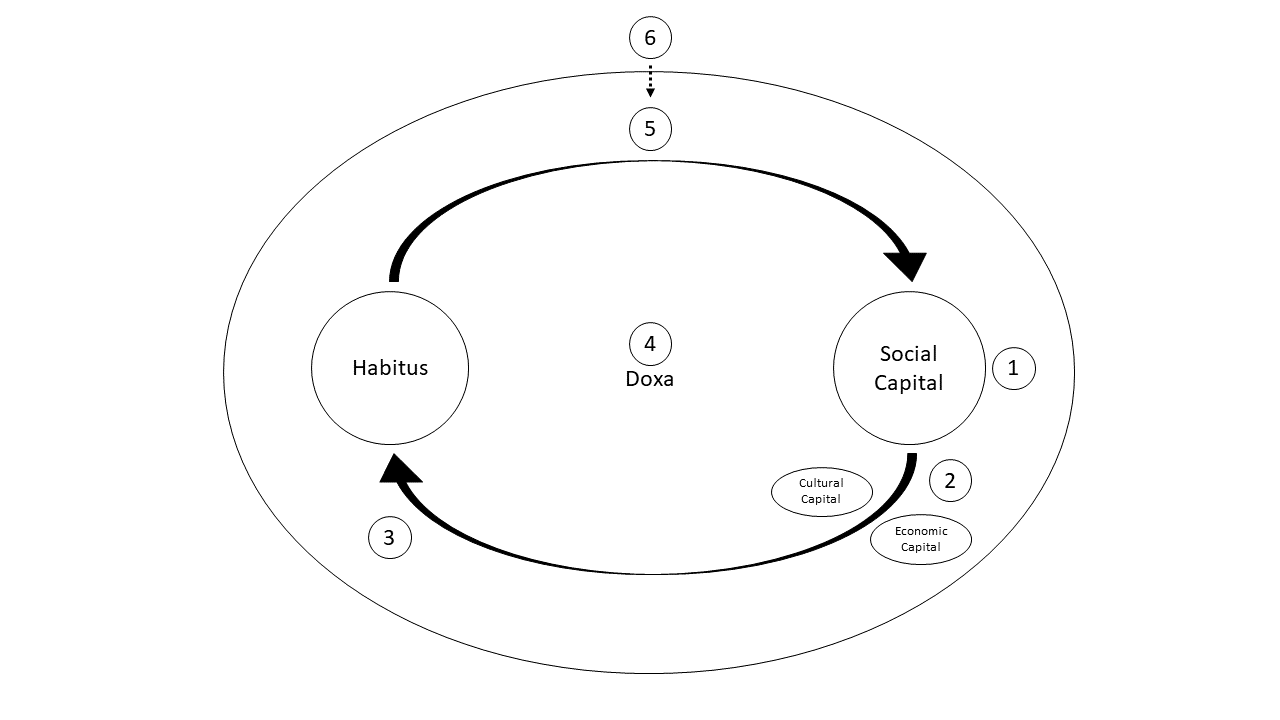
\includegraphics[width=\textwidth]{C5 - Understanding Capital Accumulation/HabitusSocCap_TheoreticalModel.png}
\caption{\label{fig:HabitusSocCap_TheoreticalModel_C7}\textbf{Complete Theoretical Model}. The complete theoretical model. The model, informed by the described experiences of university science students, expands on the interaction between habitus and capital originally illustrated by \cite{Bourdieu1984}. The model provides a step by step description of how social capital translates into habitus transformation, and how habitus generates future capital accumulation. Step 1 refers to the initial availability of social capital for an individual. Step 2 refers to the value gained through leveraging social capital into forms of economic and cultural capital. Step 3 refers to how social capital is internalised by the individual. Step 4 refers to how habitus informs the acquisition of future social capital. 5 refers to factors outside of the individual that structure the field (by availability of capital and exchange value).}
\end{figure}

\section{1: Social Capital in the Field of University Science}
This section discusses the availability of social relationships that participants had in the field of university science. These relationships are categorised into three key groups, social capital through family connections, social capital through lecturers, and social capital through peers. 

\subsection{Direction: Increase Availability of Connections}
It may be possible to address equity issues by increasing the availability of these relationships to students who would not have access to them in their everyday life. Interventions, provided by institutional support services or groups outside of institutions, can mobilise structural changes in the field by increasing the availability of connections. 

For participants in the current study, those who held connections with people who had careers in science (e.g., family members, friends, mentors, lecturers) or experience of university appeared to be the most at home at university. Students who do not have access to these forms of social capital may struggle to envision different careers in science, and what is required to progress in the field. It may be possible to address these issues by increasing the availability of these relationships to students who would not have access to them in their everyday life. As Patrick argued: ``If I just got someone to talk to me when I was young to get me interested in computer science I think that would help.'' (Patrick). Interventions, provided by institutional support services or groups outside of institutions, can mobilise structural changes in the field by increasing the availability of connections. Participants in the current study recalled their own experiences with support groups. For example, Belvia noted how a Women in Computer Science group could aid her in getting her CV out to companies. Many of the participants in the current study gained information about prospective fields through university open days, with this commonly being cited as an important influence in sparking aspirations. 

\section{2: Leveraging Social Capital}
The value of social capital is derived from the economic and cultural capital that can be mobilised through connections with others. These resources may provide students with advantages in supporting their learning and providing student access to information about the field. 


\subsection{Direction: Place Value on Alternative Forms of Cultural Capital}


\section{3: Internalising Capital}
The capital that students accrue in university science not only provides access to resources, but it can also influences the way that students see themselves in the field. Capital, which determines students position in the field, is internalised by students via their habitus, which establishes the students disposition towards the field \cite{Bourdieu1992}. Students who hold high levels of social capital may feel an affinity with the field and see progression to university as a path already drawn out. While some participants found developing relationships with those with power in the field normal, others participants did not make full use of connections as they found it ``nerve-wracking'', their lecturers ``distant'' or intimidating. 


\subsection{Direction: Educator Service Training}
Support services can facilitate students' development of social capital by providing learning environments that are welcoming. This is particularly important in classroom settings, where poor pedagogy can reduce student engagement with course content or cause students to  drop out of courses \cite{russell2011factors}. Efforts to train university teachers can improve student outcomes \cite{gibbs2004impact}, while research from New Zealand suggests that improving the cultural competence of teachers may be especially important for students who are from marginalised groups \cite{ikiua2019pasifika} and/or have English as a second language \cite{campbell2008asian}. Reframing the student-teacher relationship so it is more student-focused \cite{gibbs2004impact} and culturally responsive \cite{ikiua2019pasifika} may reduce the ``distance'' felt by students learning science at university.  




\section{4: Doxa (Societal Discourses)}
Outside of the of the social relationships that students hold, general discourses in society influence the development of habitus.

\subsection{Direction: Provide Counterspaces}


Universities may also seek to serve marginalised students by providing safe, culturally inclusive environments that combat negative doxa. \cite{mayeda2014you} describes how support services offered to M\={a}ori and Pasifika students can act as counter spaces where students can learn in a culturally inclusive environment away from judgement from Pakeha/European peers and teachers. In these spaces, students can experience a learning environment free from doxa. However, as Hakeem recalled, combating the doxa of the field must also be followed with other forms of support: \blockquote{Tu\={a}kana was good but they had the angle of destroying the stereotype for Pacific Islanders, like people normally think you are lazy and all that... it didn't feel that there was much focus on actually living, just getting into uni and getting used to just the basic kind of things, getting used to uni} Beyond combating doxa, support services can provide physical spaces that can help students facilitate connections: \blockquote{The MAPAS students... always hang around the MAPAS house so I just ask those guys. They are always helpful to answer questions from the first years} (Sean). For M\={a}ori and Pasifika students, support services may also provide extra voluntary tutorials that teach in a culturally responsive manner. As Chloe highlighted, Tu\={a}kana offered an environment where ``we all teach one another content or everyone is happy to work with each other...  it is not so cliquey''. Providing this environment can facilitate the formation of social relationships and help develop a supportive group identity. As Lily pointed out: \blockquote{we always sit together as a group during lectures and that and we all support each other through our learning and we help each other out if we don’t understand things, have little study groups. Whereas I’m not sure if the rest of the students in the course feel that way potentially because everyone is competing to get into med. So there is less ability to trust each other as students, but yeah not that same kind of willingness to help between other students}. The social capital that students gain through support services is valuable, not only because it provides academic support, but also because it provides a new norm that runs counter to the culture of independence and competition that is common in university science.

\section{5: Generating Social Capital}
The future acquisition of social capital is informed by habitus.

\subsection{Direction: Reduce the Perceived Power Imbalance}
While students may feel intimated by lecturers due to the power that they wield, counter spaces may also offer students opportunities to engage with them on a more level footing. Patrick found that being a part of Tu\={a}kana open doors: ``the lecturers are really helpful... if you have any questions or anything just go to them and then being part of the Tu\={a}kana programme is really helpful as well people to help you''. As Chloe argued, Tu\={a}kana ``removes that barrier very early'' between lecturers and students. With increased social capital, students have more sources of knowledge on the culture of the fields in which they participate in. This knowledge can inform students perceptions on how they are likely to be treated if they pursue careers in certain fields. These connections can aid students transition to university science by informing them on the content knowledge required to progress in the field. As Lily described, the Hikitia Te Ora course, a preparatory year for M\={a}ori and Pacific students going into first year health science, helped her fill gaps in her knowledge whilst also allowing her to familiarise herself with independent learning that university typically values: \blockquote{I think in terms of confidence it has given me the kind of time to be able to settle myself into some sort of routines and get an idea of what I need, things that I need to think about that I didn't need to when I was staying at home}. 


\section{6: Institutional Habitus}
The cycle is impacted on by interventions operating in the field, which themselves are directed by an institutional habitus.


\subsection{Direction: Equity Charters and Movements}


\section{Conclusion}


